\pgfplotsset{table/search path={Chapters/Glycerol/Figures},}
\graphicspath{{Chapters/Glycerol/Figures/}}
\chapter{The $\alpha$-Relaxation Dynamics of Glycerol}
\label{chap:Glycerol}

Glycerol (\ce{C3H8O3}) is a small triol molecule consisting of a three-carbon backbone with a hydroxyl group attached to each carbon. The presence of these three hydroxyl (\ce{-OH}) groups enables extensive intermolecular hydrogen bonding, leading to the formation of a dynamically evolving network structure. In addition to hydrogen bonding, weaker van der Waals interactions are also present, though they play a secondary role in determining the liquid's structure and dynamics at atmospheric pressure.

\begin{figure}[H]
	\centering
	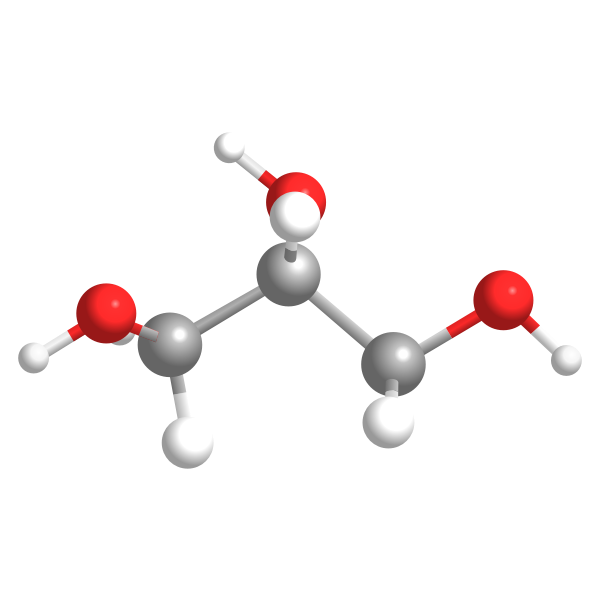
\includegraphics[width=0.35\linewidth]{Glycerol-molecule.png}
	\caption{Molecular structure of glycerol, highlighting the three hydroxyl groups responsible for hydrogen bonding.}
	\label{fig:glycerol_structure}
\end{figure}

At ambient pressure, glycerol exhibits a melting point of approximately 291~K, a boiling point near 563~K \cite{NIST_glycerol}, and a glass transition temperature $T_g \approx 190~\text{K}$ \cite[p.~6]{Angell1985}. The ability of glycerol to form multiple hydrogen bonds gives rise to a disordered network of competing local configurations and associated geometric frustration, which inhibits crystallization and makes it an excellent glass former and a model system for studying glassy dynamics.

As a hydrogen-bonding liquid, glycerol exhibits more complex behavior than simple van der Waals systems such as cumene discussed in \chap\nolinebreak \ref{chap:PCS}. In particular, the pressure dependence of fragility in hydrogen-bonded liquids has been a topic of significant interest over the past twenty-five years. Whereas most molecular liquids exhibit either decreasing fragility with increasing pressure or relatively weak pressure dependence, glycerol and similar hydrogen-bonded systems have been observed to show an increase in fragility at low to moderate pressures. This behavior is generally attributed to the influence of the hydrogen-bonding network under compression, whereas at sufficiently high pressures, where such bonding is strongly suppressed, one would expect a return toward dynamics more typical of simple van der Waals liquids \nolinebreak\cite{Casalini,Patkowski,Pronin}.

This chapter explores the current state of the literature on this topic and applies a new model to the dynamics of glycerol over a wide range of pressures and temperatures using literature data obtained through multiple experimental methods. In addition, $T_g(P)$ data, obtained \via the \tgp method described in \sect \ref{sec:IGPintro}, are used to constrain the analysis. The efficacy of viscosity data obtained by Cook \etal, which has come under some scrutiny, is reassessed, and the resulting thermodynamic scaling behavior is compared with previous literature results. Finally, a more precise measure of the pressure dependence of fragility in glycerol is presented.

\section{Earlier Works Regarding Glycerol Dynamics}

As previously asserted, glycerol is one of the most widely studied glass-forming systems, with the temperature dependence of its viscosity being investigated as far back as 1926 in the work of Tammann and Hesse \nolinebreak\cite{Tammann}.  However the modern history of glycerol, as relevant to this work, arguably begins with Davidson and Cole's investigation of the temperature dependence of the dielectric relaxation in glycerol circa 1951 \nolinebreak\cite{Davidson}.  Davidson and Cole found that not all associated liquids can be modeled with a simple single-relaxation or Debye equation as shown in \eqn\nolinebreak \ref{eqn:DebyeDielectric} \nolinebreak\cite{Debye}.  

\begin{equation}
\epsilon^*=\epsilon_\infty+\frac{\epsilon_0-\epsilon_\infty}{ 1+i\omega\tau_{0} },
\label{eqn:DebyeDielectric}
\end{equation}

 \noindent where $\epsilon_\infty$ and $\epsilon_0$ are the susceptibilities in the infinite-frequency and steady-state limits respectively.  Though 1-propanol was found to be well described by a simple Debye relationship, glycerol exhibited a higher degree of dispersion as vitrification accelerates and required unrealistically small values for its molecular volume in order for the observed relaxation time to conform to that predicted by the Debye hydrodynamic model for hard spheres.  Davidson and Cole correctly surmised that this was due to the existence of additional modes of relaxation available to glycerol that simply cannot exist for the simpler and more rigid 1-propanol molecule. To deal with this anomalous dielectric dispersion, Davidson and Cole suggested modeling such associated systems with the empirically derived "skewed" Debye like model 

\begin{equation}
\epsilon^*=\epsilon_\infty+\frac{\epsilon_0-\epsilon_\infty}{\left ( 1+i\omega\tau_{0} \right )^{\beta}},
\label{eqn:EmpiricalDielectric}
\end{equation}

\noindent where $\beta$ is the ''skewing parameter.'' Note that \eqn \ref{eqn:EmpiricalDielectric} reduces to \eqn \ref{eqn:DebyeDielectric} when $\beta=1$.  Starting with Cole and Cole, it became common in the literature of this time to plot the real \vs  imaginary components of this empirical expression as would have been common for the analysis of an analogous RC circuit\cite{Cole}. With regards to complex susceptibility, in the context of dielectric spectroscopy, the real part of \eqn \nolinebreak \ref{eqn:EmpiricalDielectric} corresponds to the non-dissipative component and the imaginary part to the dissipative component.  This can be modeled, for a simple Debye relaxation where $\beta=1$, in terms of a three component RC circuit as follows:

\begin{figure}[!htbp]
	\centering
	\begin{tikzpicture}
	
	\draw[->,line width=2pt] (0,0)--(10,0) node[anchor=north west] {$Re\left[Z\right]$} node[midway] (C) {};
	\draw[<->,very thick] (1,-.5)--(9,-.5) node[midway,anchor=north] {$R_0-R_\infty$};
	\draw[->,line width=2pt] (0,0)--(0,5) node[anchor=south east] {$-Im\left[Z\right]$};
	\draw[thick] (9,0) arc (0:180:4) node[midway] (A) {};
	\draw[->,very thick] (9,0) arc (0:45:4) node[anchor=south west] {$\omega$} node[anchor=west] (F) {};
	\node[above=0.5cm of A] (B) {$\omega\tau=1$};
	\draw[->,very thick] (B)--(A);
	\draw[->,very thick] (0,0)--(F) node[midway, anchor=south, rotate=20] {$Z\left(\omega\right)$};
	
	\draw (9,3) to[sinusoidal voltage source] (9,5) -- (11,5) to[C] (11,3) to[R](9,3);
	\draw (11,5) -- (13,5) to[R] (13,3) -- (11,3);
 	\draw (13.25,4) node[anchor=north,rotate=90]{$\left(R_0-R_\infty\right)$};
	\draw (10,2.75) node[anchor=north]{$R_\infty$};
		
	\end{tikzpicture}

	\caption{A system with a frequency dependent susceptibility and a single characteristic relaxation time $\tau$ driven at a given frequency $\omega$ can be modeled as an RC circuit as show here in the upper right corner. The complex impedance will be of the form $Z\left(\omega\right)=R_\infty+\frac{R_0-R_\infty}{1+i\omega\tau}$ which is functionally identical to the dielectric susceptibility of the simple Debye relaxation of \eqn\nolinebreak \ref{eqn:DebyeDielectric}.  Though the component which plays the role of irreversible dissipation is reversed in the case of the RC circuit above, both complex dielectric relaxation and this analogous electrical impedance will exhibit maximum dissipation at resonance where $\omega\tau=1$. }  
	\label{figure:ColeColePlot}
\end{figure}

\noindent Note that the magnitude of impedance will progress from $R_0$ to $R_\infty$ as the driving frequency is increased from $\omega=0$ to $\omega\rightarrow\infty$.  The impedance of the two limiting cases, $R_0$ and $R_\infty$, are analogous to the limiting values of the dielectric susceptibility $\epsilon_0$ and $\epsilon_\infty$ from \eqn\nolinebreak \ref{eqn:DebyeDielectric}, respectively. 

As previously mentioned, the Cole-Davidson model described by \eqn\nolinebreak \ref{eqn:EmpiricalDielectric} above may be described as a "skewed" Debye model when $0<\beta<1$ as it results in a distortion of the corresponding Cole-Cole plot.  An example of such a skewed plot of glycerol where $\beta=0.6$ and n-propanol where $\beta\approx1$, as obtained by Davidson, is shown below.  More importantly, Davidson provides a closed form expression for this distribution of simple Debye relaxations, first calculated by Fuoss and Kirkwood to describe dipole moments in polymers, which give rise to the Cole-Davidson model of \eqn\nolinebreak \ref{eqn:EmpiricalDielectric} and this is described in more detail in \chap\nolinebreak \ref{chap:PCS} \nolinebreak\cite{Fuoss}. For now, we assert that this skewing of the dielectric dispersion, increasing as the value of $\beta$ decreases, corresponds to a broader distribution of Debye-like relaxation processes.

\graphicspath{{Chapters/Glycerol/Figures/}}

\begin{figure}[!htbp]
	\begin{minipage}[t]{.45\textwidth}
	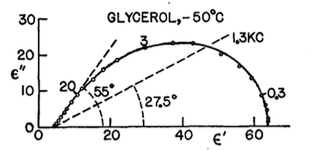
\includegraphics[width=\textwidth]{glycerolcole.png}
	\end{minipage}\hfill
	\begin{minipage}[t]{.1\textwidth}
	\end{minipage}\hfill
	\begin{minipage}[t]{.45\textwidth}
	\includegraphics[width=\textwidth]{nprop.png}
	\end{minipage}
	\caption{Cole-Cole plots of glycerol and n-propanol data (points).  Solid lines represent fits to the Cole-Davidson model of \eqn\nolinebreak \ref{eqn:EmpiricalDielectric} with beta-values of $0.6$ and $\approx 1$, respectively \protect\nolinebreak\cite{Davidson}.}  
	\label{figure:glcyerolcolecole}
	
\end{figure}

Davidson and Cole  also noted that the value of $\beta$ is essentially constant at ambient pressure over a temperature range from $40\;\si{\degreeCelsius}$ to $75\;\si{\degreeCelsius}$.  The implications of this being that the general structure of the distribution of relaxation modes is constant over a range of temperatures for which the dynamics of said relaxations are changing by at least six orders of magnitude.   Similar results have been found for many systems over the years and for such systems, this is known as time-temperature superposition.  More recently, the same has been found to hold over significant pressure ranges as well, in which case it is referred to as time-temperature-pressure superposition.  We found such results for Cumene, are described in \chap\nolinebreak \ref{chap:PCS}\textemdash$\beta$ being essentially constant over a wide range of temperature and pressure.

Though Davidson and Cole only considered the isobaric behavior of glycerol relaxation as a function of temperature, their contribution here provided some of the first data that could be used to estimate fragility\textemdash at least at atmospheric pressure. They demonstrated that the strong temperature dependence of glycerol relaxation is poorly described, even over this moderate temperature range, by a classical Arrhenius rate equation but was well fit, within experimental uncertainty, by the more empirical Vogel-Tammann-Fulcher (VTF) equation previously described by \eqn \ref{eqn:VTFintro} and first proposed by Tammann and Hesse to describe glycerol viscosity as a function of temperature \nolinebreak \cite{Tammann}.  Furthermore, they provided a closed form expression for the implied distribution of simple Debye relaxations underlying Cole-Davidson \eqn\nolinebreak \ref{eqn:EmpiricalDielectric} above.  Finally, they noted that the average molecular relaxation time of this distribution for glycerol would correspond to "hard-sphere" molecular dimensions, as provided by the classic Debye hydrodynamic theory, that are far too small to be physically realistic for glycerol, \eg, $1\times10^{-25}\;\si{\centi\meter\cubed}$, implying the existence of additional relaxation modes involving reorientation of molecular sub-units.  This observation was particularly significant, as it motivated the development and application of free-volume models for viscosity and structural relaxation upon which much of this chapter will rely.  Due to the importance of free-volume in this chapter and throughout the literature, particularly with regards to modeling viscosity of systems beyond ambient pressure, a discussion and derivation of the free-volume model will be provided in \sect\nolinebreak \ref{sec:freeVolume}.

Throughout the 1960s, work began to emerge within the literature probing viscosity and structural relaxation of glycerol beyond ambient pressure.  One of the first to appear was published in 1964 by McDuffie and Kelly where data for both viscosity, \via a rolling ball viscometer, and relaxation data, \via dielectric loss spectroscopy, were obtained \cite{McDuffie}. These methods were described previously in \sect \ref{sec:rolling_ball} and \sect \ref{sec:FRAintro}, respectively.  McDuffie and Kelly obtained viscosity data over three separate isotherms and dielectric relaxation data over a fourth which collectively covered a very small temperature range of $\Delta T=20 \;\si{\degreeCelsius}$, however, they extended these isotherms over what was, at the time, a very large range of pressure from ambient up to $4\;\si{\kilo\bar}$.  Beyond simply publishing some of the first high-pressure data for glycerol viscosity, McDuffie and Kelly's major contribution in this work was to show that neither the pressure nor temperature dependence of viscosity for glycerol was well described by the Eyring rate theory commonly used at the time and which will be described in the following section.  Also of considerable interest is that the free-volume model, described in \sect\nolinebreak \ref{sec:freeVolume}, was shown by McDuffie and Kelly to yield a compressibility for glycerol that is not congruent with high-pressure values derived from ultrasonic probes. They showed that the implementation of pressure-independent thermal expansion coefficients within the free-volume model leads to an overestimation of the pressure dependence of viscosity.  However these discrepancies were quickly addressed the following year, in 1966, by Matheson \nolinebreak\cite{Matheson}.  His arguably obvious approach was simply to apply a quadratic model to account for the pressure dependence of $\nu_{m}$ in the free-volume expression (\eqn\nolinebreak \ref{eqn:expandedViscosity}) from \sect\nolinebreak \ref{sec:freeVolumederive}.  An identical approach was used to describe the temperature dependence of several other liquids; however, the limited temperature range in McDuffie and Kelly's data was insufficient to meaningfully constrain a quadratic temperature dependence of $\nu_{m}$ in glycerol.  Still, in effectively addressing the shortcomings of early free-volume models exposed by McDufffie and Kelly \via extending the model beyond ambient pressure, Matheson's contribution was very significant. What Matheson was in want of, and what was conspicuously lacking in the literature up to this point, would be carefully collected data for glycerol viscosity or structural relaxation spanning a large temperature and pressure range.

This data gap was quickly filled by Johari and Whalley in the early 1970s with the publication of a highly cited study reporting dielectric susceptibility measurements of glycerol spanning a dynamic range of six decades \nolinebreak\cite{JohariWhalley}. Notably, their measurements extend to pressures as high as $53\;\si{\kilo\bar}$, comparable to those accessible in modern diamond anvil cell experiments, making this work a rare early example of high-pressure glassy dynamics measurements at such extremes. Their data also span a significantly broader range of temperature and pressure than previous studies, from ambient conditions to $53\;\si{\kilo\bar}$ and $-55\;\si{\degreeCelsius}$ to $84\;\si{\degreeCelsius}$, respectively.

At lower temperatures, Johari and Whalley were able to probe the relaxation dynamics of glycerol very near the glass transition. At higher temperatures, above $T = 250\;\si{\kelvin}$, their data fall approximately three decades short of approaching the glass transition. Nevertheless, the overall quality of the data has proven to be exceptional, enabling investigations into the pressure dependence of parameters such as $\beta$, defined in \eqn\nolinebreak \ref{eqn:EmpiricalDielectric}, and, later, fragility.

While the extent of their pressure range is remarkable, the accuracy of the data at the highest pressures was difficult to assess given the experimental limitations of high-pressure techniques available at the time. In this context, the incorporation of $T_g(P)$ data from the literature through the \tgp method developed in our laboratory provides a means to assess the consistency of these high-pressure measurements within a unified thermodynamic framework. As such, this work has served as a foundational reference for subsequent studies of glycerol and other glass-forming systems, with numerous citations in the literature, including those examining the pressure dependence of fragility \nolinebreak\cite{Johari2,Paluch,Forsman,Pawlus}.

Around a decade later, in 1986, Forsman \etal published a paper also probing dielectric relaxation of glycerol up to pressures of 10~kbar \nolinebreak \cite{Forsman}.  They had the advantage of nearly a decade of advancement in instrumentation and thus were able to probe significantly faster relaxations, up to $13\;\si{\mega\hertz}$.  However, these works provided relatively limited additional data, and the accessible pressure and temperature ranges were already largely covered by the earlier measurements of Johari and Whalley. While extending to faster relaxation times, such data do not substantially enhance subsequent analyses of fragility following its formal introduction by Angell, which are primarily governed by behavior near the glass transition. Though Forsman was focused more on the broadening of the loss peak as a function of pressure and furthers the discussion of many-body relaxation theory to account for deviations of the loss spectra from Debye theory, this work is worthy of mention here as it references several other papers providing data for glycerol relaxation collected over several decades.

Another work worthy of mention would be the work published by Demoulin in the early 70's \nolinebreak\cite{Demoulin}.  Though data was only taken at ambient pressure and low temperatures, Demoulin probed glycerol relaxations directly in the time domain \via photon correlation spectroscopy as described in \sect\nolinebreak \ref{sec:PCSintro}.  Though his data was confined to a relatively limited dynamic range, as autocorrelators of this era were among the first and significantly slower than those currently commercially available, with the aid of ultrasonic measurements a reasonable dynamic range was obtained.  The aim of Demoulin was not to extend the dynamic range of data available for glycerol relaxation, but rather to prove the efficacy of digital photon correlation spectroscopy as a probe of relaxation dynamics over what was an exceedingly large dynamic range for the time.  In \chap\nolinebreak \ref{chap:PCS}, a method for extending this probe into the range of very high pressures will be presented.  It is interesting here to note that, though the data obtained \via photon correlation spectroscopy is in the time domain, the Cole-Davidson distribution, being used pervasively throughout the literature to describe the dynamics of structural relaxation probed \via dielectric spectroscopy and ultrasonics methods, is most naturally expressed in terms of frequency.  This work was published before that of Lindsey and Patterson, which worked out a simple means of translating between the Williams-Watts distribution, expressed most naturally in the time domain and commonly used to model data obtained \via photon correlation spectroscopy, and the Cole-Davidson distribution of \eqn\nolinebreak \ref{eqn:EmpiricalDielectric} \nolinebreak\cite{Lindsey}.  Thus it is not surprising that Demoulin chose to impart significant effort to fit his time-domain data to the more common, yet inconvenient, Cole-Davidson distribution so that it may be directly compared to data within the literature.  His method for accomplishing this will be extended in  \chap \nolinebreak\ref{chap:PCS}, taking advantage of modern computational tools, for exactly the same reasons.

Demoulin's method of PCS will later be well established to constitute a direct measurement of structural $\alpha$-relaxation within a glass-forming system.  However, another direct probe, this time of viscosity, was introduced in the late 1970s by Geils and Keezer \nolinebreak\cite{Geils}.  The rolling ball viscometer as a means of directly measuring viscosity \via tracking the terminal velocity of a metal ball rolling down an incline, as previously described in \sect \nolinebreak\ref{sec:rolling_ball}, certainly predated the work of Geils and Keezer, however early implementations placed great restrictions on the geometry of the viscometer requiring that the ratio of the rolling ball diameter to that of the viscometer remain in one or the other limiting extremes\textemdash either rolling without slipping down a surface of the viscometer or lacking any significant interaction with the confining surfaces \nolinebreak\cite{Sutterby,Hubbard}.  Geils and Keezer worked out the means of accounting for the correction factors associated with wall effects for this method, allowing for greater flexibility in experimental design to allow for temperature and potentially pressure control, drastically increasing its efficacy as a probe for viscosity of glass-forming systems.  

\section{Reduction of extrapolation error in fragility measurements from pressure-limited data \via implementation of \tgp}

	Viscosity measurements at elevated pressure for glycerol up to about $4\;\si{\kilo\bar}$, first obtained by McDuffie and Kelly, was reported in the Journal of Chemical Physics in 1964 \nolinebreak\cite{McDuffie}.  This pressure range was significantly extended by just under an order of magnitude \via the work of Cook \etal in 1993 and 1994 implementing a diamond anvil cell viscometer attached to a centrifuge \nolinebreak\cite{Cook,Cook2}.  The data of Cook \etal were then used to investigate the pressure dependence of fragility  over this domain and appeared to show a trend of steadily increasing fragility from approximately $m\approx 55$ ($m^*=3.2$) at ambient pressure up to $m\approx 170$ ($m^*=13.6$) at $3\;\si{\giga\pascal}$ as shown in \fig \nolinebreak \ref{figure:CookFrag}.
	
	\pgfplotsset{table/search path={Chapters/glycerol/Figures},}
	\begin{figure}
		\centering
		\resizebox{0.85\textwidth}{!}{%
			\begin{minipage}[t]{.46\textwidth}
				\centering
				\begin{tikzpicture} 
					\begin{axis}[
						ylabel={$m^*=\nicefrac{\frac{\partial \ln(\eta) }{\partial \left(\nicefrac{T_g}{T}\right)}}{\ln\left( \frac{\eta_g}{ \eta_\infty}\right )}$},
						xlabel={Pressure ($\si{\giga\pascal}$)},
						xmin=0, xmax=3.5,
						ymin=0, ymax=20,
						xtick={0,.5,1,1.5,2,2.5,3,3.5},
						ytick={4,8,12,16,20},
						ymajorgrids=true,
						grid style=dashed,
						]
						\addplot+[only marks, mark=square,error bars/.cd, y dir=both,y explicit]
						coordinates { 
							(0,3.195) +- (0,.132) 
							(.202077,3.445) +- (0,.435) 
							(.405465,3.945) +- (0,1.8) 
							(.605676,4.521) +- (0,1.53) 
							(.79953,5.144) +- (0,2.256)
							(1.006097,5.8055) +- (0,2.576)
							(1.196773,6.467) +- (0,3.157)
							(1.396984,7.1272) +- (0,3.7655)
							(1.600372,7.7049) +- (0,5.129)
							(1.800583,8.468) +- (0,7.1188)
							(1.997615,9.207) +- (0,9.5487)
							(2.201004,10.048) +- (0,12.786)
							(2.404392,10.937) +- (0,17.356)
							(2.598247,11.802) +- (0,22.653)
							(2.804813,12.714) +- (0,29.424)
							(3.01138,13.569) +- (0,36.895)
						};
						\addplot+[red, only marks, mark=triangle,error bars/.cd, y dir=both,y explicit]
						coordinates {
							(.697836,5.499) +- (0,1.04) 
							(1.298467,5.927) +- (0,.6921)
						};
					\end{axis} 
				\end{tikzpicture}
			\end{minipage}
			\hspace{0.04\textwidth}
			\begin{minipage}[t]{.46\textwidth}
				\centering
				\begin{tikzpicture} 
					\begin{axis}[
						ylabel={$\nicefrac{\ln\left(\frac{\eta}{\eta_\infty}\right)} {\ln\left(\frac{\eta_g}{\eta_\infty}\right)}$},
						xlabel={Temperature ($\nicefrac{T_g}{T}$)},
						xmin=0, xmax=1,
						ymin=0, ymax=1,
						xtick={0,0.2,0.4,0.6,0.8,1},
						ytick={0.2,0.4,0.6,0.8,1},
						ymajorgrids=false,
						grid style=dashed,
						legend style={at={(0.325,.95)}},
						]
						
						\draw[dashed,thick] (0,0)--(1,1);
						\draw[dashed, thick] plot [smooth] coordinates {(0,0) (.1,.00722) (.2,.01609) (.3,.02727) (.4,.04179) (.5,.0614) (.6,.08936) (.7,.13243) (.8,.20741) (.9,.37059) (.95,.55417) (1,1)};
						\node[rotate=43.5] at (0.45,.5) {Strong};
						\node[rotate=10] at (0.3,.075) {Fragile};
						
						\addplot table [only marks,x=a, y=b, col sep=comma] {0GPAglycerol.csv};
						\addlegendentry{{\scriptsize 0.0 \;\si{\giga\pascal}}}
						\addplot table [only marks,x=a, y=b, col sep=comma] {04GPAglycerol.csv};
						\addlegendentry{{\scriptsize 0.4 \;\si{\giga\pascal}}}
						\addplot table [only marks,x=a, y=b, col sep=comma] {13GPAglycerol.csv};
						\addlegendentry{{\scriptsize 1.3 \;\si{\giga\pascal}}}
						\addplot table [only marks,x=a, y=b, col sep=comma] {3GPAglycerol.csv};
						\addlegendentry{{\scriptsize 3.0 \;\si{\giga\pascal}}}
						
					\end{axis} 
				\end{tikzpicture}
			\end{minipage}%
		}
		
		\caption{Left: the calculations of Cook \etal for the isobaric fragility of glycerol as a function of pressure with the glass transition defined at $10^{15}$ centipoise. Note that these values have been scaled to reflect our redefinition of fragility as defined in \eqn\nolinebreak\ref{eqn:scaledfragility}. This scaling of fragility is trivially accomplished as Cook \etal conveniently provides their fit parameters. The more precise values ({\color{red}$\triangle$}) were obtained from pseudoisobaric data runs of Cook \etal. Right: Angell plots for Cook \etal's 0.4, 1.3, and 3.0 \si{\giga\pascal} pseudoisobars \protect\nolinebreak\cite{Cook2}. The 0.0 \si{\giga\pascal} isobar data is from Laughlin's 1969 Ph.D. thesis \protect\nolinebreak\cite{Laughlin} although all values plotted here were directly extracted from Cook \etal's published figures.}
		\label{figure:CookFrag}
	\end{figure}  
	
	\noindent Note that, though the definition of fragility provided by \eqn\nolinebreak \ref{eqn:scaledfragility}  is arguably more physically meaningful, it may be convenient for the sake of literature comparisons to express some fragilities in terms of the more classical definition of \eqn\nolinebreak \ref{eqn:fragility}.  Thus to alleviate any confusion we will adopt a consistent notation of $m$ and $m^*$ to indicate the classical fragility of \eqn\nolinebreak \ref{eqn:fragility} and the scaled fragility of \eqn\nolinebreak \ref{eqn:scaledfragility}, respectively.  Returning now to \fig \nolinebreak \ref{figure:CookFrag}, note the excessive error associated with these fragility calculations arising from the necessity to extrapolate the VTF model over several orders of magnitude up to the glass transition.  The fact that this trend towards extreme fragility is not in satisfactory agreement with subsequent publications, particularly at elevated pressures, and the excessive error implying that the fragility measurements at high-pressure are essentially meaningless has led to the Cook \etal data being generally under-emphasized.  Paluch \etal drew attention to these concerns as well as the fact that several of the viscosity measurements were made near the melt temperature, $T_m$, where VTF model extrapolations are known to be unreliable \nolinebreak\cite{Paluch}.  The fundamental limitation for Cook \etal was that rolling ball viscometry, even when implemented within a centrifuge, can only measure viscosities up to on the order of $10^9cP$\textemdash \ie, as much as six orders of magnitude away from the glass transition at which fragility is assessed.  The data of Cook \etal, even with these concerns, does show strong support for an increasing trend in fragility with pressure up to around $2\;\si{\giga\pascal}$, which is not unexpected for a hydrogen bonding liquid where increasing fragility can be explained as arising from the diminished free-volume inhibiting hydrogen bonding.  Beyond approximately $2\;\si{\giga\pascal}$, the uncertainties in these fragilities obtained from propagating the errors in the fit parameters of the VTF equation seems to render the actual values of fragility statistically meaningless. Though the assessment of Cook \textit{et al.}, that the fragility continues to increase with pressure beyond this point, may have been somewhat compelling—given that the measurements follow a well-defined linear regression and that their standard Angell plots (shown here as modified Angell plots on the right side of \fig~4.4) appear to exhibit increasing curvature with pressure—the higher-pressure data are dubious, to say the least. Not only are the associated uncertainties excessive, but by $P = 3.0\;\si{\giga\pascal}$ glycerol has already reached a fragility of $m \approx 170$ ($m^* = 13.6$), \ie, near the upper limit of fragility observed in glass-forming liquids.  This linear trend in fragility certainly cannot continue indefinitely yet, at a pressure of $3\;\si{\giga\pascal}$, there is no indication of departing from said trend. 
	
	\pgfplotsset{table/search path={Chapters/Glycerol/SupportingFiles},}
	\begin{figure}[!htbp]
		\centering
		\begin{minipage}[t]{.45\textwidth}
			\centering
			\begin{tikzpicture} 
				\begin{axis}[
					samples=100,
					title={\parbox{\textwidth}{\centering\small $1.3\;\si{\giga\pascal}$ Scaled Angell Plot}},
					width=\linewidth,
					ylabel={$\nicefrac{\log\left(\frac{\eta}{\eta_\infty}\right)} {\log\left(\frac{\eta_g}{\eta_\infty}\right)}$},
					xlabel={Temperature $\left(\nicefrac{T_g}{T}\right)$},
					xmin=0, xmax=1.1,
					ymin=0, ymax=1.1,
					xtick={.2,.4,.6,.8,1},
					ytick={0,.2,.4,.6,.8,1},
					ymajorgrids=true,
					grid style=dashed,
					legend style={at={(0,1)},nodes={scale=.75,transform shape}, anchor=north west}
					]
					
					\addplot expression[domain=0:1.1, very thick, dashed,mark=none, Green] {.0554175*((-7.011+19.05*156.29/(227.81/x-156.29))/2.302585+3.044838613)};
					\addlegendentry{{\scriptsize \tgp}};
					\addplot expression[domain=0:1.1, very thick, solid,mark=none, Green] {.0641*((-1.378+6.629*206.496/(244.61/x-206.496))/2.302585+0.5984578)};
					\addlegendentry{{\scriptsize w/o \tgp}};
					
					\addplot [only marks, mark options={color=Green}] table [x=xmod, y=ymod, col sep=comma] {CookSystemicMissPlots.csv};
					\addplot [only marks, mark options={color=Green,fill=white}] table [x=xmodtgp, y=ymodtgp, col sep=comma] {CookSystemicMissPlots.csv};
					
				\end{axis} 
			\end{tikzpicture}
		\end{minipage}\hfill
		\begin{minipage}[t]{.05\textwidth}
		\end{minipage}\hfill
		\begin{minipage}[t]{.45\textwidth}
			\centering
			\begin{tikzpicture}
				\begin{axis}[
					samples=100,
					title={\parbox{\textwidth}{\centering\small Systemic Error in \tgp Extrapolations}},
					width=\linewidth,
					ylabel={$\log_{10}(\eta)$ (cP)},
					xlabel={Temperature ($\si{\kelvin}$)},
					xmin=150, xmax=400,
					ymin=0, ymax=18,
					xtick={200,300,400},
					ytick={0,2,4,6,8,10,12,14,16,18},
					ymajorgrids=true,
					grid style=dashed,
					unbounded coords=discard,
					legend style={at={(1,1)},nodes={scale=.75,transform shape}, anchor=north east}
					]
					
					\addplot [only marks, mark options={color=Red}] table [x=x0GPA, y=y0GPA, col sep=comma] {CookSystemicMissPlotsLog.csv};
					\addlegendentry{{\scriptsize $0.0\;\si{\giga\pascal}$}};
					
					\addplot [only marks, mark options={color=Orange},mark=diamond*] table [x=x025GPA, y=y025GPA, col sep=comma] {CookSystemicMissPlotsLog.csv};
					\addlegendentry{{\scriptsize $.25\;\si{\giga\pascal}$}}
					
					\addplot [only marks, mark options={color=YellowOrange},mark=triangle*] table [x=x07GPA, y=y07GPA, col sep=comma] {CookSystemicMissPlotsLog.csv};
					\addlegendentry{{\scriptsize $.70\;\si{\giga\pascal}$}}
					
					\addplot [only marks, mark options={color=YellowGreen},mark=square*] table [x=x1GPA, y=y1GPA, col sep=comma] {CookSystemicMissPlotsLog.csv};
					\addlegendentry{{\scriptsize $1.0\;\si{\giga\pascal}$}}
					
					\addplot [only marks, mark options={color=Green}] table [x=x13GPA, y=y13GPA, col sep=comma] {CookSystemicMissPlotsLog.csv};
					\addlegendentry{{\scriptsize $1.3\;\si{\giga\pascal}$}}
					
					\addplot  [only marks, mark options={color=BlueGreen},mark=diamond*] table [x=x17GPA, y=y17GPA, col sep=comma] {CookSystemicMissPlotsLog.csv};
					\addlegendentry{{\scriptsize $1.7\;\si{\giga\pascal}$}}
					
					\addplot [only marks, mark options={color=Blue},mark=triangle*] table [x=x25GPA, y=y25GPA, col sep=comma] {CookSystemicMissPlotsLog.csv};
					\addlegendentry{{\scriptsize $2.5\;\si{\giga\pascal}$}}
					
					\addplot [only marks, mark options={color=Violet},mark=square*] table [x=x3GPA, y=y3GPA, col sep=comma] {CookSystemicMissPlotsLog.csv};
					\addlegendentry{{\scriptsize $3.0\;\si{\giga\pascal}$}}
					
					\addplot expression[domain=150:400, very thick, solid,mark=none, Red] {(-6.143+18.012*124.904/(x-124.904))/2.302585093}; %0 GPa
					\addplot expression[domain=150:400, very thick, solid,mark=none, Orange] {(-5.625+16.574*136.265/(x-136.265))/2.302585093}; %0.25 GPa
					\addplot expression[domain=200:400, very thick, solid,mark=none, YellowOrange] {(-3.908+10.987*170.013/(x-170.013))/2.302585093}; %0.7 GPa
					\addplot expression[domain=200:400, very thick, solid,mark=none, YellowGreen] {(-2.623+8.38*190.157/(x-190.157))/2.302585093}; %1 GPa
					\addplot expression[domain=210:400, very thick, solid,mark=none, Green] {(-1.378+6.629*206.496/(x-206.496))/2.302585093}; %1.3 GPa
					\addplot expression[domain=230:400, very thick, solid,mark=none, BlueGreen] {(0.167+5.136*223.088/(x-223.088))/2.302585093}; %1.7 GPa
					\addplot expression[domain=250:400, very thick, solid,mark=none, Blue] {(2.867+3.619*244.082/(x-244.082))/2.302585093}; %2.5 GPa
					\addplot expression[domain=255:400, very thick, solid,mark=none, Violet] {(4.348+3.151*252.212/(x-252.212))/2.302585093}; %3 GPa
					
				\end{axis} 
			\end{tikzpicture}
		\end{minipage}\hfill
		
		\caption{Left:  A scaled Angell plot of the data of Cook \etal clearly demonstrates the over-estimation of fragility occurring at $1.3\;\si{\giga\pascal}$ due to extreme extrapolation up to the glass transition that is rectified \via the inclusion of \tgp data.  The same data is provided for both the solid and dotted VTF fits\textemdash scaled accordingly to their fit parameters and the glass transition temperatures they predict.  Right: Isobaric data from Cook \etal showing the general trend of under-estimation followed by increasing over-estimation of the glass transition temperature with increasing pressure.  The \tgp method provides the isochronal data at the glass transition \protect\nolinebreak\cite{Cook2}.}\label{figure:CookMiss}
		
	\end{figure}
	
	Furthermore, it is worth noting that the $3\;\si{\giga\pascal}$ fragility shown in \fig \nolinebreak \ref{figure:CookFrag} is based on only four data points and, though it is less evident in our modified Angell plot than it would be in a classical Angell plot, it does not converge to a similar infinite temperature viscosity as do data obtained at lower pressures. It is therefore not surprising that this data might yield an excessively high fragility while having error bars that include negative values of fragility\textemdash statistically speaking this is a meaningless extrapolation.  In truth, this point should likely have been omitted from Cook \etal's analysis as it relies on only three reasonably reliable data points\textemdash the underlying data for these extrapolations are shown explicitly in \fig \nolinebreak \ref{figure:CookMiss} (right), where the limited temperature coverage of the isobaric reconstructions becomes apparent.  The $50.0\;\si{\degreeCelsius}$ data point requiring a free-volume model extrapolation of almost $1\;\si{\giga\pascal}$.  However omitting the $50.0\;\si{\degreeCelsius}$ data point would leave only the $22.5$, $75.0$, and $125.0\;\si{\degreeCelsius}$, two of which still require slight extrapolation to $3\;\si{\giga\pascal}$, and require one to perform a non-linear model fit with only three data points providing constraint to a three parameter VTF model\textemdash though technically possible, an arguably meaningless endeavor.  This was the root cause of their rapidly increasing fragility estimates\textemdash simply a lack of data to properly constrain the VTF model fits and extreme extrapolation over orders of magnitude as none of this data is within the vicinity of the glass transition.

	More recent work has made a well supported case that the fragility of glycerol increases with pressure due to a progressive inhibiting of hydrogen bonding up to approximately $2\;\si{\giga\pascal}$ at which point it levels off becoming relatively constant.  It would be reasonable to assert that Cook \etal's data, as analyzed here with further constraints using data from our lab, equally well supports this general trend of fragility.  Arguably, the analysis supports a general increasing trend in fragility as pressure increases up to approximately $2\;\si{\giga\pascal}$ even if little confidence can be put into the exact fragility values above the point that the error begins to diverge rapidly.  Beyond $2\;\si{\giga\pascal}$ little can be confidently asserted from Cook \etal's analysis however it does not contradict a constant fragility when the propagated errors are accounted for.  
	
	In order to assess the validity of Cook \etal's high-pressure data and the associated fragility, it is necessary to diminish these large error bars.  This can be accomplished by addressing one of their two primary underlying issues\textemdash extreme data extrapolation.  The \tgp process developed by our group provides a direct measurement of the glass transition as a function of pressure allowing for a re-analysis of the Cook \etal data without the need for extrapolation of the VTF model over so many orders of magnitude.  This \tgp data is provided in \app\nolinebreak \ref{app:CumeneIGP} (\tbl\nolinebreak \ref{table:IGPdataGlycerol}) along with the associated Andersson-Andersson regression fit \cite{Andersson}.  Using these values for the glass transition pressure on any given isotherm and assuming this transition to occur on an isochronal curve associated with a viscosity of $\eta=10^{15}~cP$, the data Cook \etal were refit to a classical VTF model. 	
	
	\begin{figure}[!htbp]
		\centering
		\begin{tikzpicture}
			\begin{axis}[
				width=0.82\textwidth,
				height=0.55\textwidth,
				xlabel={Pressure (\si{\giga\pascal})},
				ylabel={$T_g$ (P)},
				xmin=0.15,
				xmax=4.60,
				ymin=145,
				ymax=440,
				xtick={0.5,1.0,1.5,2.0,2.5,3.0,3.5,4.0,4.5},
				ytick={150,200,250,300,350,400,450},
				ymajorgrids=true,
				xmajorgrids=true,
				grid style=dashed,
				legend style={
					at={(0.03,0.97)},
					anchor=north west,
					draw=none,
					fill=none
				},
				tick label style={font=\small},
				label style={font=\small},
				]
				
				% Cumene IGP data points
				\addplot[
				only marks,
				mark=*,
				mark size=2.4pt
				]
				table[
				col sep=comma,
				x index=0,
				y index=1
				]{Chapters/Back_matter/Figures/CumeneTGPdata.csv};
				\addlegendentry{\tgp data}
				
				% Andersson--Andersson fit
				\addplot[
				domain=0.198:4.55,
				samples=300,
				thick
				]
				{131.145*(1 + 1.64181*x/1.21852)^(1/1.64181)};
				\addlegendentry{Andersson--Andersson fit}
				
			\end{axis}
		\end{tikzpicture}
		\caption{Cumene glass-transition temperatures obtained from \tgp measurements as a function of pressure. Points correspond to the appendix data (\app\ref{app:CumeneIGP}) were one may also find the associated Andersson--Andersson fit. It should be emphasized that the $T_g(P)$ isochrone shown here does not correspond to the conventional definition of the glass transition at $\tau_g = 100~\si{\second}$, but is instead associated with a characteristic relaxation time for this specific \tgp data that will be shown to be approximately $\tau \approx 220~\si{\second}$.}
		\label{fig:CumeneIGPAA}
	\end{figure} 
	
	Note that most of the data of Cook \etal were obtained over isotherms at varying pressures.  In order to calculate fragility, they fit five sets of isothermal viscosity data to the classic free-volume model of \eqn\nolinebreak \ref{eqn:logViscosity}.  The Tait equation of state, fit to density data provided by Bridgman \nolinebreak\cite{BridgmanGly}, was implemented to convert pressure to volume.  More details regarding the implementation of the Tait equation of state for glycerol are provided in \app\nolinebreak \ref{app:GlycerolEOS} as Cook \etal and this work use this free-volume model to obtain (mostly) interpolated isobaric data as true isobaric data is difficult to obtain experimentally given that pressures will vary significantly within the DAC under thermal expansion.  Thus it is this interpolated isobaric data that is used in the fits to the VTF model for fragility analysis. 
	
	\fig \nolinebreak \ref{figure:CookMiss} (left) provides a scaled Angell plot both excluding the \tgp glass transition point (solid) as well as the refit passing through the \tgp point (dashed) for a $1.3\;\si{\giga\pascal}$ isobar.  Note that the lower five data points associated with both the dashed and solid regressions are in fact the same data from Cook \etal\textemdash scaled according to their associated VTF fits and glass transition temperatures.  The \tgp point is also provided and is, on a scaled Angell plot, located at (1,1) by definition.  It is immediately clear that both adequately describe Cook \etal's data however omitting the \tgp data leads to a significant over-estimation of fragility.  This is associated with an over-estimation of the glass transition temperature.  \fig \nolinebreak\ref{figure:CookMiss} (right) shows eight isobaric data sets, consisting of four to five data points each, ranging left to right from $0\;\si{\giga\pascal}$ to $3\;\si{\giga\pascal}$ which are obtained from the aforementioned free-volume fits to Cook \etal's published isothermal data.  The VTF fits to this data exclude the \tgp point and thus help to demonstrate the error that arises from the extrapolation of the VTF equation.  Notice that at the lowest pressures (left most curves) there is a systematic under-estimation of the glass transition temperature due to model extrapolation.  However, as we move up in pressure (to the right of the figure) we begin to increasingly over-estimate the glass transition temperature and thus over-estimate the fragility.  This trend is what is giving rise to Cook \etal's exploding fragility measurements.

From this reassessment of the data of Cook \etal, we see a very different behavior of fragility as a function of pressure.  Though, as demonstrated in \fig \nolinebreak \ref{figure:CookProninReiser}, the calculations of fragility attained from the Cook \etal data connected \via our \tgp isochronal data were still not found to be in agreement with more recent measurements, the general trend is found to be somewhat congruent \nolinebreak\cite{Pronin,Reiser}.  It should be noted that the actual values of fragility, apart from their trend with pressure, are somewhat dependent on the viscosity at the glass transition.  Following standard practice, we let the Tg(P) transition correlate with a viscosity of $\approx 10^{15}cP$.  

\pgfplotsset{table/search path={Chapters/Glycerol/Figures},}
\begin{figure}[!htbp]
	\centering
	
	\begin{tikzpicture} 
		\begin{axis}[
			samples=100,
			title={\parbox{0.35\textwidth}{\centering Isothermal Glycerol Fragilities With Increasing Pressure}},
			width=\linewidth,
			height=10cm,
			xmin=0, xmax=5,
			ymin=40, ymax=90,
			xtick={0,1,2,3,4,5},
			ytick={40,50,60,70,80,90},
			ztick={5,10,15},
			ylabel style = {align=center},
			ylabel={Pronin/Reiser \etal Fragility $m_t$},
			ymajorgrids=true,
			grid style=dashed,
			legend style={at={(1,0)},anchor=south east}
			]
			
			\addplot [blue, only marks, mark=square,error bars/.cd, y dir=both,y explicit] table [x=xcook, y=ycook, y error plus=maxcook, y error minus=mincook, col sep=comma] {FragilityComparison.csv};
			\addlegendentry{{\scriptsize Cook \etal \cite{Cook2}}}
			
			\draw[black,dashed, thick] (2,40)--(2,90);
			\draw[black,dashed, thick] (3,40)--(3,90);
			\draw[black,very thick, ->] (2.85,55)--(3,55);
			\draw[black,very thick, ->] (2.15,55)--(2,55);
			\node[] at (2.5,55) {\parbox{0.15\textwidth}{\centering H-Bonding Suppression}};
			
			\addplot+[red,only marks, mark=triangle,error bars/.cd, y dir=both,y explicit]
			coordinates { 
				(0,50.72324)    +- (0,1.938) 
				(1.426686,63.16297)    +- (0,3.0665)
				(2.170432,71.81292)    +- (0,5.063)  
				(2.464173,71.4947)    +- (0,4.918) 
				(2.966801,70.25072)    +- (0,2.95)
				(2.966979,69.1514)    +- (0,2.95)
				(3.599749,73.63549)    +- (0,3.0087) 
				(4.002432,75.05304)    +- (0,2.89296) 
				(4.468517,74.64802)    +- (0,6.914) 
				(4.54875,73.80906)    +- (0,7.985)      
			};
			\addlegendentry{{\scriptsize Pronin \cite{Pronin}}}
			
			\addplot+[green,only marks, mark=star,error bars/.cd, y dir=both,y explicit]
			coordinates { 
				(0,53.03688)    +- (0,3) 
				(.1,52.32513)    +- (0,3)
				(.2,53.18672)    +- (0,3)  
				(.3,53.13989)    +- (0,3) 
				(.4,54.01085)    +- (0,3)
				(.5,55.05975)    +- (0,3)
				(.6,56.05246)    +- (0,3) 
				(.7,57.07326)    +- (0,3)        
			};
			\addlegendentry{{\scriptsize Reiser \etal \cite{Reiser}}}
			
			\addplot+[no marks,very thick, black] {46.664493+27.40865/(1+4.496047*e^(-1.40425*x))};
			\addlegendentry{{\scriptsize Guide}}
			
			\addplot+[no marks,very thick, dashed, black] {0.43429*(38.964-.299834*(x*10))*(1+(38.964-.299834*(x*10))/(19.0451-.625929*(x*10)+.00644846*(x*10)^2-.00000616589*(x*10)^3))};
			\addlegendentry{{\scriptsize Surface}}
			
		\end{axis} 
	\end{tikzpicture}
	
	\caption{The fragility measurements calculated from classic VTF fits to Cook \etal's viscosity data corrected \via the inclusion of our \tgp glass transition point ($\color{blue}\square$) are shown above to be no longer wholly incongruent with more recent work. A smooth curve is included as a guide to the eye through the Pronin ($\color{red}\triangle$) and Reiser \etal ($\color{green}\star$) data, suggesting that the increase in fragility appears to saturate between 2 and 3 $\si{\giga\pascal}$ as originally asserted by Paluch \protect\nolinebreak\cite{Paluch} and Pawlus \protect\nolinebreak\cite{Pawlus}. The fragilities of Cook \etal retain relatively large uncertainties, thus cannot reflect accurately the fine behavior of fragility as a function of pressure, yet do seem to reflect this fragility increase between 2 and 3 $\si{\giga\pascal}$. A reasonable trend-line is provided that falls within all error bars.} 
	\label{figure:CookProninReiser}
\end{figure}

A quick assessment of \fig \nolinebreak \ref{figure:CookFragIGP} might suggest a decrease in fragility from ambient pressure up to approximately $1.5\;\si{\giga\pascal}$, and the propagated uncertainties derived from the covariance of the VTF fit parameters appear to indicate statistical significance in this trend. However, these error bars reflect only the internal consistency of the VTF fitting procedure and do not account for more fundamental sources of uncertainty.

In this regime, the determination of fragility relies on extrapolation of the VTF form over many decades in relaxation time, with minimal experimental constraint near the glass transition. While the inclusion of the \tgp isochron constrains the location of $T_g$, it provides only a single point in the vicinity of the transition and therefore does not meaningfully constrain the slope of the VTF function from which the fragility is derived. As a result, the calculated fragility remains strongly dependent on both the assumed validity of the VTF form and the underlying Cook \etal\ dataset. Consequently, the apparent decrease in fragility should not be interpreted as physically robust. Rather, it reflects the limitations of the available data and fitting procedure, which are insufficient to reliably capture the evolution of fragility.

\pgfplotsset{table/search path={Chapters/glycerol/Figures},}
\begin{figure}[!htbp]
	\centering
	\resizebox{0.8\textwidth}{!}{%
		\begin{minipage}[t]{.475\textwidth}		
			\begin{tikzpicture} 
				\begin{axis}[
					ylabel={$m^*=\nicefrac{\frac{\partial \ln(\eta) }{\partial \left(\nicefrac{T_g}{T}\right)}}{\ln\left( \frac{\eta_g}{ \eta_\infty}\right )}$},
					xlabel={Pressure ($\si{\giga\pascal}$)},
					xmin=0, xmax=3.5,
					ymin=1, ymax=8,
					xtick={0,.5,1,1.5,2,2.5,3,3.5},
					ytick={2,3,4,5,6,7,8},
					ymajorgrids=true,
					grid style=dashed
					]
					\addplot+[only marks, mark=square,error bars/.cd, y dir=both,y explicit]
					coordinates { 
						(0.7,3.512883)    +- (0,.168) 
						(1.3,3.181076)    +- (0,.546)
						(0,3.958805)    +- (0,.064)  
						(2,4.16682)    +- (0,.51) 
						(2.5,4.922827)    +- (0,.468)
						(.25,3.801)    +- (0,.0535) 
						(1,3.339)    +- (0,.328) 
						(1.7,4.083887)    +- (0,.213) 
						(0.5,3.638201)    +- (0,.088)
						(3,5.98637)    +- (0,2.547)  
					};
				\end{axis} 
			\end{tikzpicture}
		\end{minipage}
		\hspace{0.05\textwidth}
		\begin{minipage}[t]{.475\textwidth}		
			\begin{tikzpicture} 
				\pgfplotsset{set layers}
				%
				\begin{axis}[
					xmin=0,xmax=3.5,
					ymin=-10,ymax=20,
					ytick={-5,0,5,10,15,20},
					axis y line*=left,
					ymajorgrids=true,
					grid style=dashed,
					xlabel={Pressure ($\si{\giga\pascal}$)},
					ylabel style = {align=center},
					ylabel={$\Delta T_g$ ($\si{\kelvin}$)}
					]
					\addplot +[mark=square] table [only marks,x=a, y=b, col sep=comma] {RegressionError.csv};
				\end{axis}
				%
				\begin{axis}[
					xmin=0,xmax=3.5,
					ymin=-2,ymax=10,
					axis y line*=right,
					axis x line=none,
					ylabel style = {align=center},
					ylabel={$\Delta m^*$},
					]
					\addplot +[mark=triangle] table [only marks,x=c, y=d, col sep=comma] {RegressionError.csv};
				\end{axis}
			\end{tikzpicture}
		\end{minipage}\hfill
	}
	\caption{Left:  Scaled fragility as a function of pressure derived from classic VTF fits to the data of Cook \etal with the glass transition point included as determined \via our \tgp isochron.  Right: The error in terms of under or over-estimation of the glass transition temperature, $\Delta T_g$, due to extreme extrapolation of the VTF model as demonstrated in \fig \nolinebreak \ref{figure:CookMiss}, is provided ($\color{blue}\square$) along with error in scaled fragility ($\color{blue}\triangle$) calculated from these extrapolated models. } \label{figure:CookFragIGP}
\end{figure}

The right side of \fig \nolinebreak \ref{figure:CookFragIGP} shows the under or over estimation of the glass transition temperature as a function of pressure derived from the classic VTF fits to the data of Cook \etal without the \tgp isochronal data. The initial under-estimation of the glass transition temperature for the two lowest pressures is followed by a trend of increasing over-estimation up to about $1.7\;\si{\giga\pascal}$ where we continue to over-estimate the transition temperature, albeit to an increasingly lesser degree.  However the error in fragility associated with this over-estimation in glass transition temperature continues to increase in a fairly linear fashion leading to the excessively high fragilities at increased pressure observed by Cook \etal in \fig \nolinebreak \ref{figure:CookFrag}.

It is worth noting here that, though viscosity data of Cook \etal was predominately taken along isotherms as this was experimentally favorable, they did manage to obtain two pseudo-isobaric runs at $0.7$ and $1.3\;\si{\giga\pascal}$ on which they then used interpolation between free-volume fits to their isothermal data to correct for slight deviations of pressure.  Though this process was extremely time intensive, it did provide them with two isobaric runs over a large temperature range addressing the issue of insufficient data points.  It should be noted, however, that these data are still limited to well below the glass transition.  Due to the larger number of data points associated with these pseudo-isobaric runs, the error associated with the fragility estimations are significantly smaller and these two points are included ($\color{red}\triangle$) in the left side of \fig \nolinebreak \ref{figure:CookFrag}.  These two higher-confidence points would alone imply a potentially constant fragility below $1.5\;\si{\giga\pascal}$\textemdash albeit at a significantly higher scaled fragility $(m^*\approx 5.7)$.  

Beyond $1.5\;\si{\giga\pascal}$ the fragility steadily increases by $\Delta m^*\approx 7.8$ and then remain approximately constant within uncertainty beyond $2.5$ to $3\;\si{\giga\pascal}$ before rapidly diverging due to extrapolation errors again.  This general trend of increasing fragility is, in the loosest sense, in "agreement" with subsequent published works as will be demonstrated.  This leads to the conclusion that the viscosity data of Cook \etal is perhaps significantly more reliable than may have been assumed and much of its error, as perhaps expected, is predominately the result of these extrapolation issues. Our method of employing \tgp data to diminish this extrapolation error significantly decreases the error associated with these fragility estimations however it is still limited\textemdash particularly at elevated pressures.  More data is needed in the region of interest to further define the slope at the glass transition\textemdash data which has since been provided by other groups and is included in \fig \ref{figure:CookProninReiser}.    

Other methods such as photon correlation spectroscopy and dielectric loss spectroscopy certainly exist and there is no shortage of data for glycerol dynamics within the literature around the vicinity of the glass transition, though generally limited to cryogenic measurements at low pressures.  If the issues with these fragility calculations do in fact stem predominately from the lack of data in critical regions rather than the efficacy of the data itself, then supplementation of their data with other literature data in critical regions should allow accurate determinations of fragility as a function of pressure. Glycerol data taken by several different groups extend over different pressure and temperature regions and include both viscosity and $\alpha$-relaxation measurements, making glycerol a prime candidate for a surface fragility analysis, similar to what will also be done for cumene in \chap\nolinebreak \ref{chap:PCS}.  

To add further validation to Cook \etal's data at lower pressures, the same analysis method of implementing the \tgp data point to constrain the VTF fits in the vicinity of the glass transition was applied to the rolling ball data obtained by McDuffie and Kelly and the associated fragilities calculated \nolinebreak\cite{McDuffie}.  Though these fragility values were much more in line with other works implementing dynamic light scattering (Brodin \nolinebreak\cite{Brodin}), and dielectric spectroscopy (Reiser \etal \nolinebreak\cite{Reiser}, Pronin \nolinebreak\cite{Pronin}, and McDuffie and Kelly \nolinebreak \nolinebreak\cite{McDuffie}), they all follow the same general trend of constant fragility below $1\;\si{\giga\pascal}$.  The increasing trend mentioned by Pronin and Reiser \etal is simply not statistically significant.  This seems to suggest a strong increase in fragility does not occur until beyond $1\;\si{\giga\pascal}$.  This may be due to the general expected trend of decreasing fragility with increasing pressure is being approximately balanced by the early onset of hydrogen bond breaking giving rise to a relatively constant fragility in this range.

\section{Structural Relaxation Surface}

	Experimentally, it is often difficult to obtain truly isobaric data at high-pressure. When a fluid is confined within a pressure vessel or diamond--anvil cell, changes in temperature inevitably induce changes in pressure due to thermal expansion.  In their PCS measurements, Cook \etal went to considerable lengths to interpolate between data points in order to construct pseudo--isobaric data runs.  Of considerable utility, therefore, would be a framework capable of fitting relaxation data acquired over broad ranges of temperature and pressure (or specific volume) without requiring strict isobaric or, for that matter isothermal, constraints.  This motivates the development of a continuous structural--relaxation surface.

	To this end, the Andersson--Andersson constrained surface model provided in \app \ref{app:AndersonSurface} is employed, extending the classic isobaric Vogel--Tammann--Fulcher (VTF) formalism to account for pressure dependence through polynomial expansions of pressure--dependent parameters. A more rigorous mathematical development of this model is presented in \sect \ref{sec:surface}.  Here, only the essential structure of the surface and the physical constraints imposed upon it are discussed.
	
	For most liquids, a substantial body of high--quality ambient--pressure data exists in the literature, obtained using a variety of experimental probes of structural relaxation and viscosity, owing to the relative experimental accessibility of this thermodynamic region\textemdash glycerol being no exception. \fig \ref{figure:1barglycerol} presents an Angell plot of almost all atmospheric--pressure data collected for this work, together with a fit to the classic isobaric VTF model. This atmospheric-pressure isobar serves as a primary constraint for the relaxation surface.
	
	It should be noted that the Cook \etal data have been excluded from this atmospheric--pressure constraint. The \tgp point, shown on the same Angell plot at a location corresponding to $\tau = 220~\si{\second}$ as determined from thermodynamic scaling of the low--pressure \tgp data in \fig \ref{figure:GlycerolIGPLinear}, was likewise not included in the fit, though it exhibits excellent agreement with the data what was included. 
	
	At the time the atmospheric-pressure data were fit, the degree to which the intercept method of thermodynamic scaling accurately determines the isochronal value associated with the Andersson--Andersson regression of the \tgp data was not yet established.  One peripheral insight arising from the development of these surface models is the realization that, for liquids whose dynamics conform to thermodynamic scaling, this approach provides a robust means of identifying the precise isochrone represented by a given \tgp data run. Even in cases where thermodynamic scaling may not strictly apply, the atmospheric--pressure constraint provides an independent verification of this isochronal value, as the Andersson--Andersson regression through the \tgp data must intersect the atmospheric VTF isobar.
	
	The Andersson--Andersson regression through the \tgp data provides an additional constraint to be imposed on the surface construction. Specifically, the VTF expression is solved for the zero--mobility temperature $T_0$ in terms of the pressure--dependent glass--transition temperature $T_g(P)$ and subsequently reinserted into the VTF form, yielding  \eqn \ref{eqn:glycerolSurfaceModel}.  Here, $T_g(P)$ is taken from the Andersson--Andersson fit to the \tgp data provided in \app \ref{app:GlycerolIGP}.  
	This procedure results in a relaxation surface constrained both at atmospheric pressure and along an isochrone corresponding to $\tau \approx 220~\si{\second}$.
	
	The remaining four parameters comprising the coefficient vectors $\vec{d}$ and $\vec{t}$ are treated as free parameters and are determined using a Levenberg--Marquardt optimization algorithm to conform the surface to the remaining data\textemdash excluding the \tgp and 1-bar data. \fig \ref{figure:CookSurfaceFit} displays this constrained surface together with the Cook \etal data, shown for initial parameter estimates. The atmospheric isobaric constraint and the isochronal \tgp constraint are indicated by solid black curves on the surface.
	
	It is emphasized that the surface is not fit to the Cook \etal data. Because they measured viscosity directly via rolling--ball viscometry, whereas all other data in this chapter probe the structural $\alpha$--relaxation time, the decision was made to include the Cook \etal data only for qualitative comparison.  The Cook \etal viscosity data were scaled using an appropriate high--frequency shear modulus $G_\infty$ to permit comparison with the relaxation--time surface.
	
	Glycerol viscosity and relaxation data from several sources are shown, along with the Cook \etal rolling ball data obtained from within a DAC, in \fig \nolinebreak \ref{figure:GlycerolSurfaceFitWithError} \nolinebreak\cite{Brodin,McDuffie,Paluch,Pronin,Reiser}.  It is clear that data is actually in excellent agreement with other literature data further bolstering the case that the vast majority of the error within the Cook \etal fragility measurements lies in the extreme extrapolation to the glass transition.  The inclusion of the \tgp isochronal data, though addressing the issue of extrapolation to a significant extent, ultimately provides insufficient accommodation for an accurate determination of the rate of vitrification with increasing pressure in the vicinity of the glass transition, $T_g$.  More data is needed to define the slope near $T_g$ to obtain an isobaric fragility in consensus with other contributors to the literature, \ie Pronin, Paluch, \etc  
	
	In short, there never was any issue with the validity of Cook \etal's viscosity data before extrapolation.  As we will see, it is in reasonable agreement with other measurements of vitrification or associated alpha relaxation behavior.  It is only the lack of data to provide constraint to the VTF fit in key locations, specifically in the vicinity of $T_g$, that gives rise to the incongruence of the Cook \etal fragility estimations with literature values, \ie the slope in the vicinity of $T_g$ is poorly constrained.  The addition of the \tgp isochronal data is not itself sufficient to provide the necessary constraint on this slope for reliable estimations of fragility.  However, as we will here demonstrate, only one additional experimentally trivial, constraint is needed for Cook \etal's data to provide fragility values as a function of pressure in excellent agreement with the current literature consensus\textemdash an ambient isobar.  
	
		\pgfplotsset{table/search path={Chapters/glycerol/SupportingFiles},}
		\begin{figure}[!htbp]
		\resizebox{0.95\textwidth}{!}{%
		\begin{tikzpicture}
		\begin{axis}[restrict z to domain=0:18,zmax=18,zmin=0,
		width=0.9\textwidth,
		xmax=400, xmin=180,
		ymax=3, ymin=0,
		xtick={200,240,280,320,360,400},
		ytick={1,2,3},
		ztick={5,10,15},
		xlabel = Temperature $(\si{\kelvin})$,
		ylabel = Pressure  $(\si{\giga\pascal})$,
		zlabel = {$\log_{10} <\tau> (\si{\pico\second})$},
		title = {Andersson--Andersson Constrained Surface Model With Cook \etal Viscosity Data},
		]
		
		\addplot3[forget plot, only marks, scatter = false, mark options={draw=blue, fill=blue}] table [x=temp, y=pressure, z=logtau, col sep=comma] {fitsurfaceGlycerolDataCook.csv};
		
		\addplot3[no marks,very thick, scatter] table [x=temp, y=pressure, z=logtau, col sep=comma] {1BarRegression.csv};
		
		\addplot3[no marks,very thick, scatter] table [x=temp, y=pressure, z=logtau, col sep=comma] {TgpRegressionshort.csv};
		
		\addplot3[
		mesh,
		samples=23,
		samples y=31,
		domain=180:400,y domain=0:3,
		draw=black       
		]
		{(-6.0104+.176307*(y*10)+(188.376*(1+.0365618*(y*10))^(.488759)*(19.0464-.848505*(y*10)+.0222398*(y*10)^2-.000214289*(y*10)^3))/(-188.376*(1+.0365618*(y*10))^(.488759)+x+(19.0462-.848505*(y*10)+.0222398*(y*10)^2-.000214289*(y*10)^3)*x/(39.7601-.176307*(y*10))))/ln(10)
		};
		
		\end{axis}
		\end{tikzpicture}
		}
		\caption{Cook \etal's rolling ball viscosity data is here provided along with the Andersson-Andersson constrained surface model, given initial approximations for the fit parameters, described in \app\nolinebreak \ref{app:AndersonSurface}. The surface is extended to $3\;\si{\giga\pascal}$ corresponding to the highest pressures for which Cook \etal obtained data \protect\nolinebreak\cite{Cook2}. The mesh lines correspond to constant-temperature and constant-pressure slices (isotherms and isobars), spaced at 10~K and 0.1~GPa, respectively.}
		\label{figure:CookSurfaceFit}
		
	\end{figure}

\fig \nolinebreak\ref{figure:CookSurfaceFit} shows all of Cook \etal's raw viscosity data provided by reference \nolinebreak\cite{Cook2} fit to the Andersson-Andersson constrained surface model described in \app\nolinebreak \ref{app:AndersonSurface}.  The Solid black isobaric line at atmospheric pressure, through which the surface is constrained, is well described in \fig \nolinebreak \ref{figure:1barglycerol}, along with the supporting data.  This 1-bar regression was also used to define the isochrone for the \tgp curve\textemdash the second solid black line extending across the top of the surface in \fig \nolinebreak \ref{figure:CookSurfaceFit}.  The glycerol \tgp data fit to a standard Andersson-Andersson model is provided in \app\nolinebreak \ref{app:GlycerolIGP} and corresponds to an isochronal pressure-temperature relationship at $\tau\approx10^{14}\;\si{\pico\second}$ through which the surface is also constrained.  

This Andersson-Andersson constrained surface model, fit to the Cook \etal viscosity data, allows for a determination of fragility as a function of pressure in similar fashion to that obtained for cumene in \fig \nolinebreak \ref{figure:fragilityPressure}.  The resulting functional dependence of isobaric fragility is plotted as a solid black line in \fig \nolinebreak \ref{figure:CookProninReiser} above and found to be in significantly greater agreement with Pronin, Reiser \etal, and other more recent works up to $2.5\;\si{\giga\pascal}$.  This result, along with the excellent constrained surface fit, suggest that Cook \etal's data could not be lacking significantly in quality.  

	\begin{figure}[!htbp]
	\resizebox{0.95\textwidth}{!}{%
	\begin{tikzpicture}
	\begin{axis}[
	colorbar,
	point meta min=-10, 
	point meta max=20,
	restrict z to domain=0:18,zmax=18,zmin=0,
	width=0.9\textwidth,
	xmax=400, xmin=180,
	ymax=5, ymin=0,
	ytick={1,2,3,4,5},
	ztick={5,10,15},
	xlabel = $Temperature (\si{\kelvin})$,
	ylabel = $Pressure (\si{\giga\pascal})$,
	zlabel = {$Log_{10} <\eta> (cP)$},
	title = {Glycerol Relaxation Data},
	legend style={only marks, at={(0,1)},anchor=north east}
	]
	
	\addplot3[only marks, scatter, scatter src=explicit] table [x=temp, y=pressure, z=logtau, meta=error, col sep=comma] {fitsurfaceGlycerolDataCook.csv};
	\addlegendentry{{\scriptsize Cook \etal \cite{Cook2}}}
	
	\addplot3[only marks, mark=square*, scatter, scatter src=explicit] table [x=temp, y=pressure, z=logcp, meta=error, col sep=comma] {fitsurfaceGlycerolDataPaluch.csv};
	\addlegendentry{{\scriptsize Johari and Whalley \cite{JohariWhalley}}}
	
	\addplot3[only marks, mark=triangle*, scatter,scatter src=explicit] table [x=temp, y=pressure, z=logcp, meta=error, col sep=comma] {fitsurfaceGlycerolDataPronin.csv};
	\addlegendentry{{\scriptsize Pronin \cite{Pronin}}}
	
	\addplot3[only marks, mark=star, scatter, scatter src=explicit] table [x=temp, y=pressure, z=logcp, meta=error, col sep=comma] {fitsurfaceGlycerolDataReiser.csv};
	\addlegendentry{{\scriptsize Reiser \etal \cite{Reiser}}}
	
	\addplot3[only marks, mark=x, scatter, scatter src=explicit] table [x=temp, y=pressure, z=logtau, meta=error, col sep=comma] {fitsurfaceGlycerolData1bar.csv};
	\addlegendentry{{\scriptsize 1-Bar \cite{Brodin,Pronin,Ngai}}}
	
	\addplot3[only marks, mark=diamond*, scatter, scatter src=explicit] table [x=temp, y=pressure, z=logtau, meta=error, col sep=comma] {fitsurfaceGlycerolDataTgp.csv};
	\addlegendentry{{\scriptsize \tgp}}
	
	\addplot3[no marks,very thick, scatter, scatter src=explicit] table [x=temp, y=pressure, z=logtau, meta=error, col sep=comma] {1BarRegression.csv};
	
	\addplot3[no marks,very thick, scatter, scatter src=explicit] table [x=temp, y=pressure, z=logtau, meta=error, col sep=comma] {TgpRegression.csv};
	
	%\addplot3[only marks, scatter] table [x=temp, y=pressure, z=logtau, col sep=comma] {fitsurfaceGlycerolDataMcDuffie.csv};
	
	\addplot3[
	point meta=0,
	mesh,
	samples=23,
	samples y=51,
	domain=180:400,
	y domain=0:5
	]
	{
		14.3733
		- ((8.27174 + 2.44421*y - 0.153233*y^2)
		* (126.678 + 13.237*y - 0.540195*y^2 - 0.0459642*y^3))
		/(-126.678
		+ 188.376*(1 + 0.365618*y)^(0.488759)
		- 13.237*y
		+ 0.540195*y^2
		+ 0.0459642*y^3)
		+ ((8.27174 + 2.44421*y - 0.153233*y^2)
		* (126.678 + 13.237*y - 0.540195*y^2 - 0.0459642*y^3))
		/(-126.678
		- 13.237*y
		+ 0.540195*y^2
		+ 0.0459642*y^3
		+ x)
	};
	
	
	\end{axis}
	
	\node[] at (15,-.5) {$\% Error$}; 
	\end{tikzpicture}
	}
	\caption{The surface shown corresponds to the model described in \app\nolinebreak\ref{app:AndersonSurface}, fit to a compilation of glycerol relaxation data from Johari and Whalley, Pronin, and Reiser \etal. The Cook \etal, \tgp, and atmospheric data were not included in the fit, but are represented on the surface. Data points are colored by their percent deviation from the fitted surface, highlighting systematic trends in the residuals. The mesh lines correspond to constant-temperature and constant-pressure slices (isotherms and isobars), spaced at 10~K and 0.1~GPa, respectively.}
	\label{figure:GlycerolSurfaceFitWithError}
	
\end{figure} 

In \fig \ref{figure:GlycerolSurfaceFitWithError} we have the model described in \app\nolinebreak \ref{app:AndersonSurface} fit to a large selection of glycerol relaxation data from multiple contributers, including Pronin \etal \cite{Pronin}, Johari and Whalley \cite{JohariWhalley}, and Reiser \etal \cite{Reiser}.  The same \tgp and 1-bar constraint was imposed here as was implemented in \fig\nolinebreak \ref{figure:CookSurfaceFit}.  The color scale represents percent deviation of the data from the surface.  Note how the high-pressure Pronin data begins to diverge from the surface, approaching an error as high as $20\%$.  This data was still included in the fit as it conforms well to the surface at higher temperatures and lower viscosities\textemdash only tending away from the surface in a region where the \tgp constraint does not allow the data significant influence over the fit parameters.

\fig \nolinebreak\ref{figure:GlycerolSurfaceFitWithError} shows the same Andersson-Andersson constrained surface model fit to a larger selection of literature data including Cook \etal's rolling ball viscosity data.  The same \tgp and atmospheric constraints are applied.  Here the Actual \tgp data is provided on the surface yet not included in the fit.  It is found that Cook \etal's rolling ball viscosity data is in excellent agreement with other works including Johari and Whalley, Pronin, Paluch, and Reiser \etal thus we must conclude that the Cook \etal data is very reliable\textemdash the issue of increasingly overestimated fragility arising predominately from extreme extrapolation \nolinebreak\cite{Johari,Paluch,Pronin,Reiser}.  It should be noted that the four isobaric data sets extracted from Pronin's \fig 3 in reference \nolinebreak \cite{Pronin} do trend increasingly above the fit surface at higher pressures yet agree with Cook \etal and others at lower pressures.  The toroidal pressure cell used by Pronin and described in reference \cite{Khvostantsev} may not have provided a hydrostatic sample to the degree that was assumed\textemdash a scenario which would certainly explain the data's increasing divergence from the \tgp isochrone at higher pressures and lower temperatures as the glass transition is approached.  The Pronin isobars are still in reasonable agreement with Cook \etal's data at higher temperatures where hydrostatic conditions are assured, even at the highest pressure.  However this data was included as it does not heavily effect the surface at lower pressures where it is in reasonable agreement with the rest of the data yet allows us to extend this fit surface up to $5\;\si{\giga\pascal}$.  Thus it should be assumed that our calculated fragility above $3\;\si{\giga\pascal}$ may have reasonable error associated with it and any fine structure is not of high confidence.  It should be noted that this Pronin data could be replaced with DPCS measurements at high pressure near the glass transition just as was done with cumene. Molecular simulations may provide high-pressure fast dynamics at extreme temperatures.  

\begin{figure}[!htbp]
	\centering
	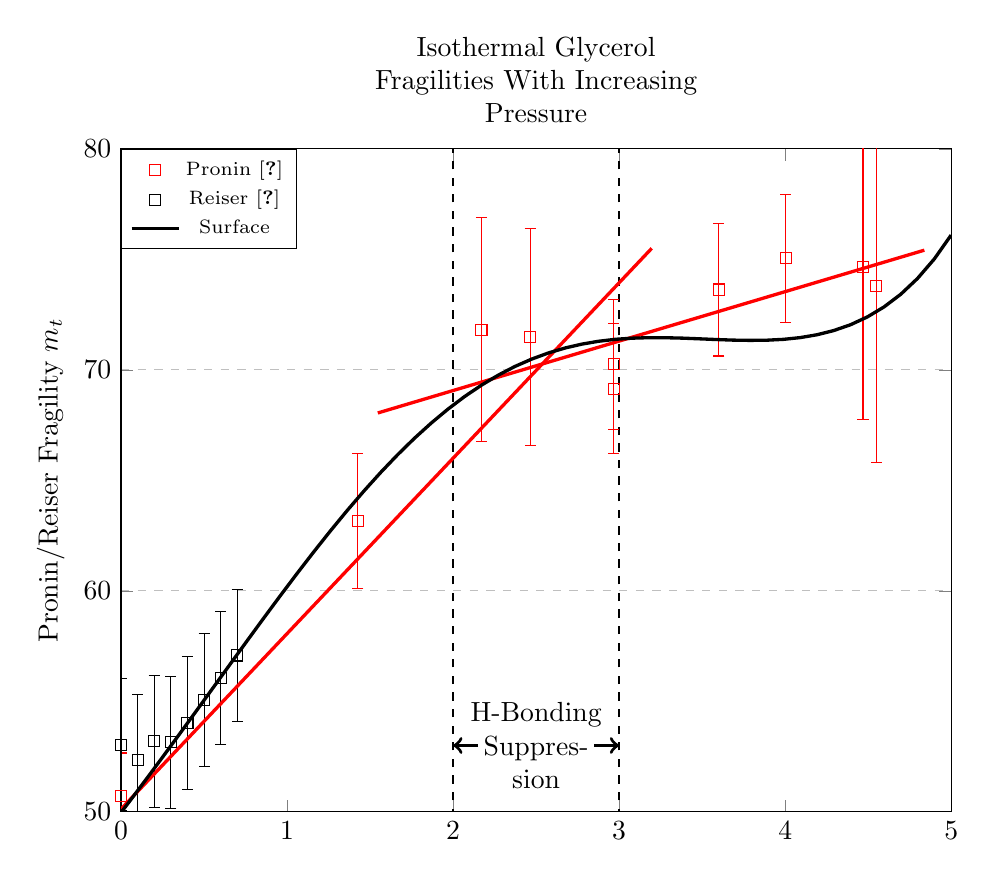
\begin{tikzpicture} 
	
	\begin{axis}[
	title={\parbox{0.35\textwidth}{\centering Isothermal Glycerol Fragilities With Increasing Pressure}},
	samples=100,
	width=\linewidth,
	height=10cm,
	xmin=0, xmax=5,
	ymin=50, ymax=80,
	xtick={0,1,2,3,4,5},
	ytick={50,60,70,80},
	ylabel style = {align=center},
	ylabel={Pronin/Reiser \etal Fragility $m_t$},
	ymajorgrids=true,
	grid style=dashed,
	legend style={at={(0,1)},anchor=north west}
	]
	
	\draw[black,dashed, thick] (2,40)--(2,80);
	\draw[black,dashed, thick] (3,40)--(3,80);
	\draw[black,very thick, ->] (2.85,53)--(3,53);
	\draw[black,very thick, ->] (2.15,53)--(2,53);
	\node[] at (2.5,53) {\parbox{0.15\textwidth}{\centering H-Bonding Suppression}};
	
	\addplot+[red,only marks, mark=square,error bars/.cd, y dir=both,y explicit]
	coordinates { 
		(0,50.72324)    +- (0,1.938) 
		(1.426686,63.16297)    +- (0,3.0665)
		(2.170432,71.81292)    +- (0,5.063)  
		(2.464173,71.4947)    +- (0,4.918) 
		(2.966801,70.25072)    +- (0,2.95)
		(2.966979,69.1514)    +- (0,2.95)
		(3.599749,73.63549)    +- (0,3.0087) 
		(4.002432,75.05304)    +- (0,2.89296) 
		(4.468517,74.64802)    +- (0,6.914) 
		(4.54875,73.80906)    +- (0,7.985)      
	};
	\addlegendentry{{\scriptsize Pronin \cite{Pronin}}}
	
	\addplot+[black,only marks, mark=square,error bars/.cd, y dir=both,y explicit]
	coordinates { 
		(0,53.03688)    +- (0,3) 
		(.1,52.32513)    +- (0,3)
		(.2,53.18672)    +- (0,3)  
		(.3,53.13989)    +- (0,3) 
		(.4,54.01085)    +- (0,3)
		(.5,55.05975)    +- (0,3)
		(.6,56.05246)    +- (0,3) 
		(.7,57.07326)    +- (0,3)        
	};
	\addlegendentry{{\scriptsize Reiser \etal \cite{Reiser}}}
	
	\draw[red, very thick] (0,50.1228) -- (3.195876,75.49795);
	\draw[red, very thick] (1.546392,68.049) -- (4.838,75.4161);
	
	\addplot+[no marks,very thick, black] {0.434294*(38.2465-0.1569*(x*10))*(1+(38.2465-0.1569*(x*10))/(19.0462-.75566*(x*10)+.0188737*(x*10)^2-.000176531*(x*10)^3))};
	\addlegendentry{{\scriptsize Surface}}
	
	\end{axis} 
	\end{tikzpicture}
	
	\caption{Fragility estimations from Pronin ($\color{red}\square$) and Reiser \etal's ($\color{black}\square$) data are shown above.  The pressure dependence of fragility derived from isobaric temperature derivatives of the Andersson-Andersson surface model described in \app\nolinebreak \ref{app:AndersonSurface}, fit to the data of Cook \etal, Johari and Whalley, Pronin, Paluch, and Reiser \etal, is shown as a solid black line.  The upward curve in fragility approaching $5\;\si{\unit{\giga\pascal}}$ is likely a relic due to the previously discussed issues with the Pronin data at high pressure as well as the surface being generally unconstrained by data beyond this pressure. }
	\label{figure:FinalFragilities}
\end{figure}

The calculated fragility as a function of pressure arising from the Andersson-Andersson surface model from \fig \nolinebreak \ref{figure:GlycerolSurfaceFitWithError} including data from Cook \etal, Johari and Whalley, Pronin, Paluch and Reiser \etal is provided in \fig \ref{figure:FinalFragilities}\textemdash extending our fragility measurements out to $5\;\si{\giga\pascal}$.  The red lines show Pronin's original estimation of the fragility behavior with increasing pressure as was lifted directly from his \fig~4 in reference \nolinebreak \cite{Pronin}. This result shows unequivocally Cook \etal's rolling ball viscosity data to be in excellent agreement with other literature measurements of viscosity, $\eta$, and $\tau_\alpha$.  The Andersson--Andersson constrained surface model relieves us of the experimental burden of maintaining isobaric conditions during data acquisition, which is very difficult to accomplish in a diamond anvil cell. It also avoids reliance on free-volume models, where a reliable equation of state may not be available, as well as isothermal models such as the modified VTF equation of \eqn \ref{eqn:ModifiedVTFPressureClassic}, which will appear in our discussion of cumene but may not adequately capture the transition from a hydrogen-bonded liquid to one exhibiting more van der Waals behavior, such as glycerol.

\section{Equation of State and Thermodynamic Scaling} \label{sec:GlycerolScaling}

Simple van der Waals glass-forming liquids have been shown to obey density scaling, in which the relaxation dynamics conform to a single function of the form $\tau \propto (T V^\gamma)^{-1}$, where $\gamma$ is a material-dependent constant. In \sect\nolinebreak \ref{sec:tdscaling}, this behavior is demonstrated explicitly for cumene, where density scaling is found to hold over a compression approaching 29\%. In the case of a simple liquid such as cumene, the intermolecular interactions are well approximated by the Lennard--Jones potential,
\begin{equation}
	U(r)=4\epsilon\left[\left(\frac{\sigma}{r}\right)^{12}-\left(\frac{\sigma}{r}\right)^6\right],
	\label{eqn:LennardJones}
\end{equation}
for which the short-range repulsive term scales as $r^{-12}$. Because structural relaxation is governed primarily by these steep repulsive interactions at close intermolecular separation, the dynamics are expected to reflect an effective inverse power-law form dominated by this repulsive contribution.

This factor $\gamma$ has been shown to depend on the intermolecular potential energy landscape, which may be approximated as $U(r)\sim\left(\frac{\sigma}{r}\right)^{3\gamma}$, where $r$ is the spatial separation between any two molecules and $\sigma$ is a material constant \nolinebreak\cite{Roland2005RPP, Roland3,Coslovich}. Within this framework, one expects an effective scaling of the form $U(r)\sim r^{-3\gamma}$, with $3\gamma = 12$ in the limiting case of a purely inverse power-law repulsive interaction of the form $r^{-12}$. Real liquids, however, are not strictly inverse power-law systems due to the presence of attractive interactions and molecular complexity, and thus are expected to exhibit effective exponents that deviate from this ideal value. In the case of cumene $\gamma\approxeq4.77$\textemdash indicating a slightly steeper effective repulsive interaction than that of an ideal Lennard--Jones fluid. The dynamics of such liquids are therefore strongly driven by simple free-volume considerations, and thus we expect thermodynamic scaling to hold with increasing pressure, as is observed in the case of cumene.

However, in the case of strongly associated liquids such as glycerol, intermolecular interactions include directional hydrogen bonding, which introduces additional structure into the potential energy landscape beyond simple isotropic repulsion. While all intermolecular interactions depend on temperature and pressure, the presence of such directional bonding can inhibit the emergence of a single effective inverse power-law description, and thus thermodynamic scaling is not generally expected to hold in these systems. Nevertheless, several such liquids do exhibit thermodynamic scaling\textemdash at least over limited ranges of pressure and temperature, where the influence of specific interactions is reduced and the dynamics become increasingly governed by short-range repulsive forces.

Glycerol is one such example, having a measured scaling parameter within the literature in the range of $1.4\leq \gamma \leq 1.6$ \nolinebreak\cite{Reiser,Kyaw}.  This lower value for $\gamma$ is expected given that free-volume will play a reduced role in the dynamics of associated liquids as molecular mobility is no longer just a matter of thermal diffusion past nearest neighbors exhibiting van der Waals repulsion, but also will require energy to break hydrogen bonds with said neighbors.  However these values for $\gamma$ were all determined at relatively low pressures\textemdash on the order of $0.1\;\si{\mega\pascal}$, \ie, near ambient pressure.  Yet we see in \fig \ref{figure:FinalFragilities} a shift in the fragility behavior as a function of pressure occurring between $2$ and $3\;\si{\giga\pascal}$ which has been attributed to a suppression of hydrogen bonding. If hydrogen bonding between glycerol molecules is sufficiently suppressed at very high pressures, one might expect glycerol to behave much more like a simple van der Waals liquid with a scaling parameter, $\gamma$, much closer to 4 as the potential energy landscape no longer is heavily influenced by these suppressed intra-molecular interactions.  

\pgfplotsset{table/search path={Chapters/Glycerol/SupportingFiles},}
\begin{figure}[!htbp]
	\centering
	\begin{tikzpicture} 
	\begin{axis}[
	title={Thermodynamic Scaling of \tgp Isochrone},
	ylabel={Log$(T)$},
	xlabel={-Log$(V)$},
	ymin=2.25, ymax=2.55,
	xmin=-.08, xmax=.08,
	scaled x ticks=true,
	xtick scale label code/.code={},
	xlabel={$-\log(V)\;(\times 10^{-2})$},
	%xtick={0,.002,.004,.006,.008,.01},
	%ytick={0,2,4,6,8,10,12,14,16},
	width=0.9\textwidth
	]
	
	\addplot table [only marks, x=LogV, y=LogT, col sep=comma] {glycerolTGPscaling.csv};
	
	\addplot expression[domain=-.08:.04,mark=none,red]{
	1.5359*x+2.3667};

	\addplot expression[domain=0.01:0.08,mark=none,red]{
	3.6536*x+2.3155};

	\draw[black,dashed, thick] (0.01842,2.25) -- (0.01842,2.55);
	\draw[black,dashed, thick] (0.03535,2.25) -- (0.03535,2.55);
	
	\draw[black,very thick, ->] (0.01842,2.28)--(0.03535,2.28);
	\draw[black,very thick, ->] (0.03535,2.28)--(0.01842,2.28);
	\node[font = {\fontsize{8 pt}{12 pt}\selectfont}] at (0.02688,2.295) {\parbox{0.15\textwidth}{\centering H-Bonding Suppression}};
	
	\node[rotate=60] at (0.06,2.50) {\parbox{0.15\textwidth}{\centering y=3.65x+2.32}};
	
	\node[rotate=36] at (-.03,2.3) {\parbox{0.15\textwidth}{\centering y=1.54x+2.37}};
	
	\node[] at (-0.06,2.5) {\parbox{0.15\textwidth}{\centering Increasing Pressure}};
	\draw[black,line width=3pt, ->] (-0.045,2.5)--(-0.03,2.5);

	\end{axis}
		
	\end{tikzpicture}
	\caption{The linearized isochronal glycerol \tgp data shows a transition from an H-bonded liquid at low pressure with a corresponding scaling factor of $\gamma\approxeq1.54$ to a liquid which behaves more like one experiencing a simple van der Waals potential at higher pressures, where H-boding is suppressed, exhibiting a scaling factor of $\gamma\approxeq3.65$.  The region between the dotted vertical lines corresponds the region indicated in \fig \ref{figure:FinalFragilities} previously.  The intersection of the two linear regimes is self consistent with the results of Pronin at approximately $2.5\;\si{\giga\pascal}$.  It is also worthy of note that the average y-intercept of 2.35 implies a \tgp isochrone of $\tau\approx 220\;\si{\unit{\second}}$.}
	\label{figure:GlycerolIGPLinear}
\end{figure}

In \fig \ref{figure:GlycerolIGPLinear}, the glycerol \tgp data provided in \app \ref{app:GlycerolIGP} is linearized and plotted to determine the scaling parameter.  Rather than assuming thermodynamic scaling a priori, we instead test for its validity by considering the expected form
\begin{equation}
	\tau \propto (T V^\gamma)^{-1},
	\label{eqn:GlycerolScaling}
\end{equation}
which, upon rearrangement, implies
\begin{equation}
	\log(T) = -\gamma \log(V) + \mathrm{const}.
	\label{eqn:GlycerolScalingLinear}
\end{equation}
Thus, if thermodynamic scaling holds, a plot of $\log(T)$ versus $-\log(V)$ should yield a linear relationship, with the slope directly corresponding to the scaling parameter $\gamma$.

The region between the dotted lines once again corresponds to that in \fig \ref{figure:FinalFragilities}\textemdash where pressure suppression of hydrogen bonding becomes prominent.  The results are quite compelling.  Two distinct regions emerge.  At low pressure we find a scaling factor $\gamma=1.54$ consistent with literature values. At high pressures, well within the region where hydrogen bonding is assumed to be sufficiently suppressed, we find a significantly greater slope corresponding to $\gamma=3.65$ consistent with what might be expected of a simpler van der Waals liquid. A clear transition occurs between $2$ and $3\;\si{\giga\pascal}$\textemdash consistent with our fragility results from our Andersson-Andersson contained surface model as well as Pronin's analysis.

\pgfplotsset{table/search path={Chapters/Glycerol/SupportingFiles},}
\begin{figure}[!htbp]
	\centering
	\resizebox{0.95\textwidth}{!}{%
	\begin{tikzpicture} 
	\begin{axis}[
	colorbar,
	colorbar style={xshift=1cm,
		yticklabel pos=left,
		yticklabel style={anchor=east},
		rotate=0},
	title={Thermodynamic Scaling of Surface Data},
	ylabel={Log$(\eta)$},
	xlabel={$\frac{10^{-4}}{TV^\gamma}$},
	ymin=1, ymax=16,
	xmin=0.9, xmax=3,
	%xtick={0,.002,.004,.006,.008,.01},
	%ytick={0,2,4,6,8,10,12,14,16},
	width=0.9\textwidth,
	legend style={only marks, at={(0,1)},anchor=north west}
	]
	
	\addplot [scatter,point meta=explicit,point meta min={0}, point meta max={6.55}] table [only marks, x=xcook, y=ycook, meta=Pcook, col sep=comma] {glycerolTGPScaledData2.csv};
	\addlegendentry{{\scriptsize Cook \etal \cite{Cook2}}}
	
	\addplot [mark=square,scatter,point meta=explicit,point meta min={0}, point meta max={6.55}] table [only marks, x=xJandW, y=yJandW, meta=PJandW, col sep=comma] {glycerolTGPScaledData2.csv};
	\addlegendentry{{\scriptsize Johari and Whalley \cite{Johari}}}
	
	\addplot [mark=triangle,scatter,point meta=explicit,point meta min={0}, point meta max={6.55}] table [only marks, x=xpronin, y=ypronin, meta=Ppronin, col sep=comma] {glycerolTGPScaledData2.csv};
	\addlegendentry{{\scriptsize Pronin \cite{Pronin}}}
	
	\addplot [mark=star, scatter,point meta=explicit,point meta min={0}, point meta max={6.55}] table [only marks, x=xreiser, y=yreiser, meta=Preiser, col sep=comma] {glycerolTGPScaledData2.csv};
	\addlegendentry{{\scriptsize Reiser \etal \cite{Reiser}}}
			
	\addplot [mark=diamond,scatter,point meta=explicit,point meta min={0}, point meta max={6.55}] table [only marks, x=xtgp, y=ytgp, meta=Ptgp, col sep=comma] {glycerolTGPScaledData2.csv};
	\addlegendentry{{\scriptsize \tgp}}
	
	\node[rotate = 55] at (2.5,8) {\parbox{0.15\textwidth}{\centering High Pressure}};
	\node[rotate = 55] at (1.6,8) {\parbox{0.15\textwidth}{\centering Low Pressure}};
	
	\end{axis}
	
	\node[] at (15.2,-.5) {$\si{\giga\pascal}$};
	
	\end{tikzpicture}
	}

	\caption{The results of thermodynamic scaling of glycerol for all low pressure data ($<2\;\si{\giga\pascal}$) with a scaling factor of $\gamma = 1.54$ and high-pressure data ($>3\;\si{\giga\pascal}$) with a scaling factor of $\gamma = 3.65$.}
	\label{figure:GlycerolIGPScaling}
	
\end{figure}

All of the glycerol data that falls outside of the transition region between $2$ and $3\;\si{\giga\pascal}$ provided by Cook \etal, Johari and Whalley, Pronin, Reiser \etal, and our \tgp data exhibit a reasonable degree of thermodynamic scaling along one of two curves.  The results of this scaling are provided in \fig \nolinebreak \ref{figure:GlycerolIGPScaling}.  We see that all of the Cook \etal data scales nicely even well into the intermediate pressure regimen-perhaps due to the relative high temperatures allowing for molecular mobility which facilitates hydrogen bonding at these higher pressures. The Johari and Whalley data, on the other hand, is all at relatively low to intermediate temperatures and a clear pressure dependent divergence from good thermodynamic scaling is observed as pressure increases and hydrogen bonding begins to be suppressed.  All of this still relies on an extreme extrapolation of the Tait equation of state for which Bridgman only provides data up to approximately $1.2\;\si{\giga\pascal}$ however thermodynamic scaling is possible, albeit in two distinct regimens each with different scaling factor, $\gamma$.  Where hydrogen bonding is not being suppressed we find a scaling factor $\gamma=1.54$ that reflects a liquid for which free-volume plays a diminished role in the dynamics. 

Once again we note that the high-pressure data of Pronin \etal taken in the toroidal pressure cell seems to scale at lower pressures or higher temperatures however, as vitrification sets in at higher pressure the data peels away from the trend expected if thermodynamic scaling were to hold in precisely the same manner that it peeled away from the Andersson-Andersson constrained surface fit previously. It appears once again as if the reported pressures are lower than what the dynamics would imply.  As this discrepancy is occurring only at the highest pressure and in the region where vitrification is rapidly increasing, it stands to reason that they have underestimated the prominence of pressure gradients within their toroidal cell. The lower pressure data, even in the vicinity of the glass transition, scales nicely just as it conformed very well to the relaxation surface.  However as pressures increase the odds of significant pressure gradients inside the cell increases greatly.  